
\documentclass[]{slides}
\title{MIPS design}
\date{August - December 2020}

% Begin document
\begin{document}
\printpdftrue % uncomment to hide pauses
% Title slide
\begin{frame} \titlepage \end{frame}

\section{A basic \acl{uP}}
% ========================================
% 
% ========================================
\begin{frame}{Basic \ac{uP}}
  \begin{figure}
  \centering
  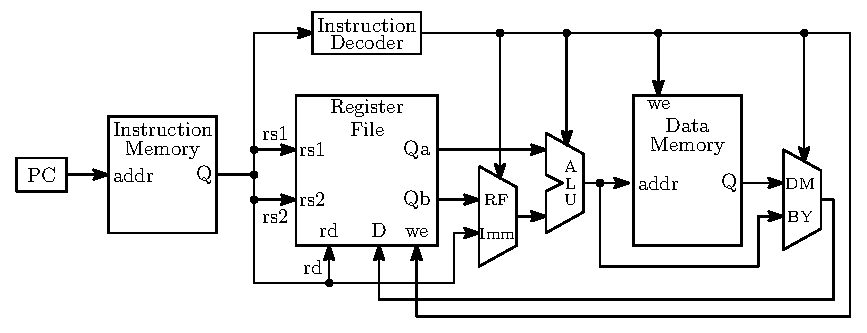
\includegraphics[width=\textwidth]{MIPS_design_basic_cpu}
  \caption{Generalised \ac{uP} schematic.}
  \label{Figure:non_pipelined_cpu}
  \end{figure}
\end{frame}

% ========================================
% 
% ========================================
\begin{frame}{Basic \ac{uP}}
  \begin{figure}
  \centering
  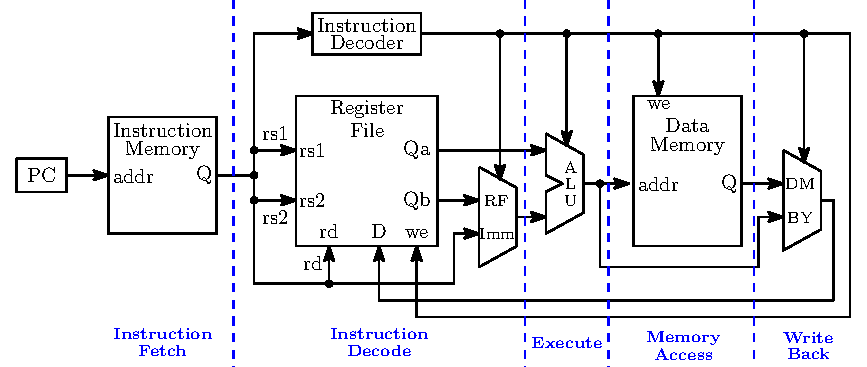
\includegraphics[width=\textwidth]{MIPS_design_basic_cpu_stages}
  \caption{Stages of a \ac{uP} cycle.}
  \label{Figure:non_pipelined_cpu_stages}
  \end{figure}
\end{frame}


% ========================================
% 
% ========================================
\begin{frame}{Stages of a basic \ac{uP} instruction cycle}
\begin{enumerate}
\item \acbf{IF}. Instructions are read from \ac{IM}.
\item \acbf{ID}. Type of operation and operands are defined.
\item \acbf{EXE}. Operands are used in order to perform arithmetic or logical operations.
\item \acbf{MEM}. Data is read/written from/to \ac{DM}.
\item \acbf{WB}. Results from \ac{EXE} or \ac{MEM} stages are written back into \ac{RF}.
\end{enumerate}
\end{frame}

% ========================================
% 
% ========================================

\section{MIPS example}
\begin{frame}{\acs{MIPS}}{}
  \begin{itemize}
  \item \ac{MIPS} is a \ac{RISC}-type \ac{uP}.
  \item \ac{MIPS} flavours could use 16, 32- or 64-bits data widths.
  \item Supports 3 main instruction types.
    \begin{itemize}
    \item R-Type for register-register operations.
    \item I-Type for immediate operations.
    \item J-Type for jump operations.
    \end{itemize}
  \end{itemize}
\end{frame}

% ========================================
% 
% ========================================
\begin{frame}{\acs{MIPS} instruction encoding}
  \begin{figure}
  \centering
  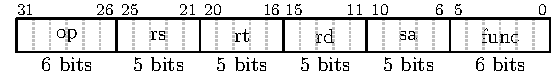
\includegraphics[width=\textwidth]{MIPS_design_encoding_1}
  \caption{Example of \acs{MIPS} encoding.}
  \label{Figure:MIPS32_encoding_1}
  \end{figure}
    \begin{itemize}
  \item \alertblue{op:} Basic operation of the instruction, traditionally called \alert{opcode}.
  \item \alertblue{rs:} First register source operand.
  \item \alertblue{rt:} Second register source operand.
  \item \alertblue{rd:} Destination register.
  \item \alertblue{sa:} Shift amount.
  \item \alertblue{func:} Function. Specifies a variant of the operation in the op field.
  \end{itemize}
\end{frame}

% ========================================
% 
% ========================================
\begin{frame}{\acs{MIPS} instruction encoding}
    \begin{itemize}
    %\item Go to www.menti.com and enter the code 31 98 66.
    %\pauseprint
    \item Considering the previous encoding
    \begin{itemize}
    \item What type(s) of addressing modes are available?
    \item How many registers can we access?
    \item Can we access data from the memory?
    \end{itemize}
    \pauseprint
    \item Since \ac{MIPS} is a \ac{RISC}, we can't simply add bits to the encoding.
    \begin{itemize}
    \item Why?
        \pauseprint
    \end{itemize}
    \item Instead, we must use the same 32-bits for accessing memory.
    \item For this purpose, some of the fields will have to be modified.
  \end{itemize}
\end{frame}

% ========================================
% 
% ========================================
\begin{frame}{\acs{MIPS} instruction encoding}
  \begin{figure}
  \centering
  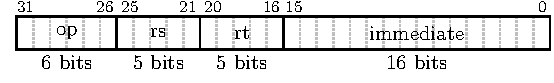
\includegraphics[width=\textwidth]{MIPS_design_encoding_2}
  \caption{Example of another \acs{MIPS} encoding.}
  \label{Figure:MIPS32_encoding_2}
  \end{figure}
  \begin{itemize}
  \item This format will allow us to access memory using a 16-bit address.
  \item This will also allow us to use immediate values (constants) for arithmetic and logical operations.
  \end{itemize}
\end{frame}

% ========================================
% 
% ========================================
\begin{frame}{\acs{MIPS} instruction encoding}
\alertblue{These are the encodings for each of the 3 main \ac{MIPS} instruction types.}
  \begin{figure}
  \centering
  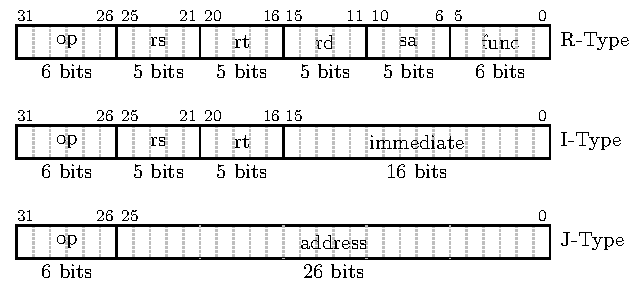
\includegraphics[width=\textwidth]{MIPS_design_instruction_types}
  \caption{\acs{MIPS}32 instruction types.}
  \label{Figure:MIPS32_instruction_types}
  \end{figure}
\end{frame}

% ========================================
% 
% ========================================
\begin{frame}{\ac{MIPS} instruction fields}
  \begin{itemize}
  \item \alertblue{op:} Basic operation of the instruction, traditionally called \alert{opcode}.
  \item \alertblue{rs:} First register source operand.
  \item \alertblue{rt:} Second register source operand.
  \item \alertblue{rd:} Destination register.
  \item \alertblue{sa:} Shift amount.
  \item \alertblue{func:} Function. Specifies a variant of the operation in the op field.
  \item \alertblue{immediate:} A value that defines an address or a constant.
  \item \alertblue{address:} An absolute address value.
  \end{itemize}
\end{frame}

% ========================================
% 
% ========================================
\begin{frame}{}
  \begin{figure}
  \centering
  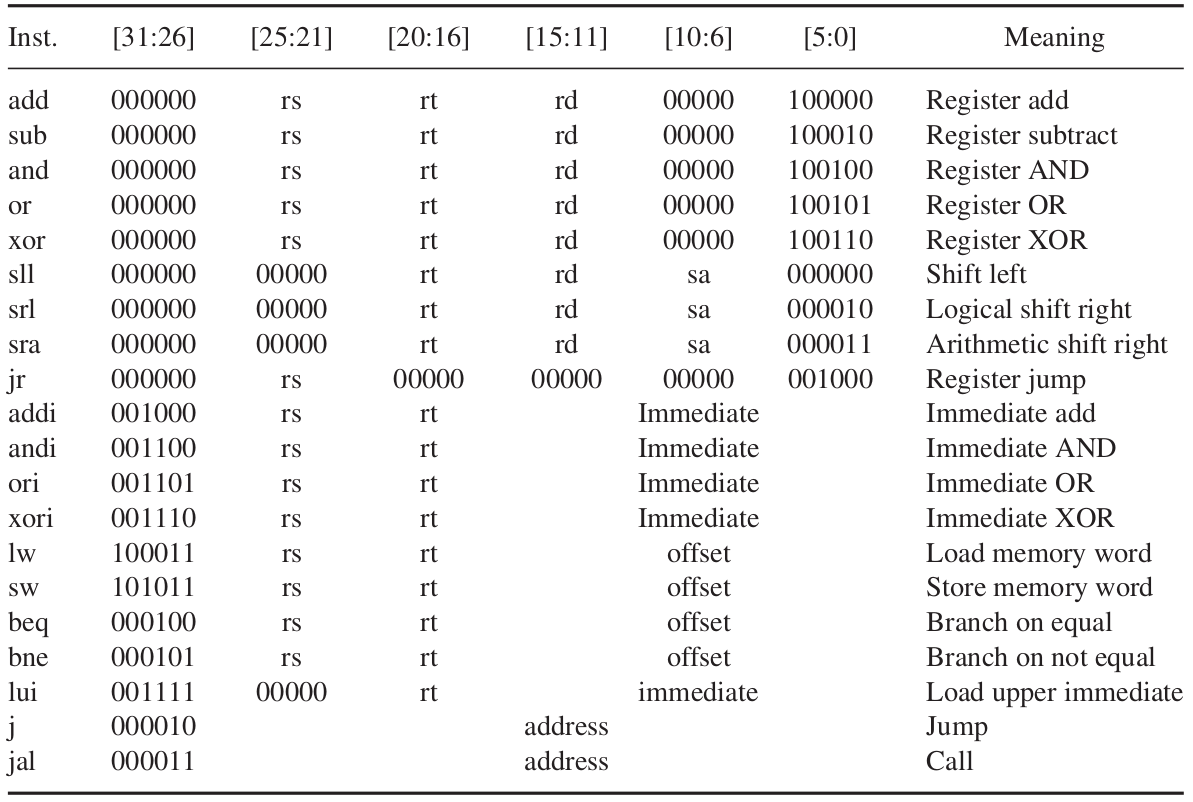
\includegraphics[scale=0.28]{MIPS_design_integer_instructions}
  \vspace{-8pt}
  \caption{\acs{MIPS}32 integer instructions.}
  \label{Figure:MIPS32_integer_instructions}
  \end{figure}
\end{frame}

% sll/srl/sra rd, rt, sa # rd <-- rt shift sa
% lui rt, immediate # rt <-- immediate << 16
% lw rt, offset(rs) # rt <-- memory[rs + offset]
% sw rt, offset(rs) # memory[rs + offset] <-- rt
% bne rs, rt, label # if (rs != rt) PC <-- label
% j target # PC <-- target
% jr rs # PC <-- rs
% ========================================
% 
% ========================================
\begin{frame}{\acs{MIPS} instruction examples}
  \begin{table}[htbp]
  \caption{MIPS instruction examples}
  \label{Table:MIPS_instruction_examples}
    \begin{tabular}{llll|l}
    \hline\hline
    \multicolumn{4}{c|}{\textbf{Instruction}} & \textbf{Meaning} \\\hline
      \code{add} & \code{rd,} & \code{rs,} & \code{rt} & \code{rd} $\leftarrow$ \code{rs + rt} \\\hline 
    \code{addi} & \code{rt,} & \code{rs,} & \code{imm} & \code{rt} $\leftarrow$ \code{rs + (sign\_ext)imm} \\\hline 
    \code{ori} & \code{rt,} & \code{rs,} & \code{imm} & \code{rt} $\leftarrow$ \code{rs | (zero\_ext)imm} \\\hline 
    \code{sra} & \code{rd,} & \code{rt,} & \code{sa} & \code{rd} $\leftarrow$ \code{rt << sa} \\\hline 
    \code{lui} & \code{rt,} & \multicolumn{2}{l|}{\code{imm}} & \code{rt} $\leftarrow$ \code{imm << 16} \\\hline 
    \code{lw} & \code{rt,} & \multicolumn{2}{l|}{\code{offset(rs)}} & \code{rt} $\leftarrow$ \code{memory[rs + offset]} \\\hline 
    \code{sw} & \code{rt,} & \multicolumn{2}{l|}{\code{offset(rs)}} & \code{memory[rs + offset]} $\leftarrow$ \code{rt} \\\hline 
    \code{bne} & \code{rs,} & \code{rt,} & \code{label} & \code{if (rs != rt) then PC} $\leftarrow$ \code{label} \\\hline
    \code{j} & \multicolumn{3}{l|}{\code{target}} & \code{PC} $\leftarrow$ \code{target} \\\hline
    \code{jr} & \multicolumn{3}{l|}{\code{rs}} & \code{PC} $\leftarrow$ \code{rs} \\\hline 
    \end{tabular}
  \end{table}
\end{frame}


\newcommand{\mipsinstA}{\code{add r4, r5, r6}\xspace}
\newcommand{\mipsinstB}{\code{sub r4, r5, r6}\xspace}
\newcommand{\mipsinstC}{\code{subu r4, r5, r6}\xspace}
\newcommand{\mipsinstD}{\code{addi r7, r8, -10}\xspace}
\newcommand{\mipsinstE}{\code{addiu r7, r8, -2}\xspace}
\newcommand{\mipsinstF}{\code{and r7, r8, r6}\xspace}
\newcommand{\mipsinstG}{\code{andi r7, r8, -1}\xspace}
\newcommand{\mipsinstH}{\code{lw r12, 100(r4)}\xspace}
\newcommand{\mipsinstI}{\code{sw r12, 100(r4)}\xspace}
\newcommand{\mipsinstJ}{\code{lw r12, -100(r4)}\xspace}
\newcommand{\mipsinstK}{\code{sw r12, -100(r4)}\xspace}
\newcommand{\mipsinstL}{\code{j 1234}\xspace}
\newcommand{\mipsinstM}{\code{jr r23}\xspace}

\newcommand{\coloropcode}[1]{\alertblue{#1}\xspace}
\newcommand{\colorrs}[1]{\alertdarkgreen{#1}\xspace}
\newcommand{\colorrt}[1]{\alertmagenta{#1}\xspace}
\newcommand{\colorrd}[1]{\alertviolet{#1}\xspace}
\newcommand{\colorsa}[1]{\alertcyan{#1}\xspace}
\newcommand{\colorfunc}[1]{\alertred{#1}\xspace}
\newcommand{\colorimmediate}[1]{\alertcyan{#1}\xspace}

\newcommand{\crt}{\colorrt{rt}}
\newcommand{\crs}{\colorrs{rs}}
\newcommand{\crd}{\colorrd{rd}}
\newcommand{\cimmediate}{\colorimmediate{immediate}}
\newcommand{\caddress}{\colorimmediate{address}}

% ========================================
% 
% ========================================
\begin{frame}{MIPS encoding example}
Use \textcolor{blue}{\href{http://www.mrc.uidaho.edu/mrc/people/jff/digital/MIPSir.html}{\ac{MIPS} encoding format}} in order to translate the following assembler code to machine code.
\begin{enumerate}
\item \mipsinstA
\item \mipsinstB
\item \mipsinstC
\item \mipsinstD
\item \mipsinstE
\item \mipsinstF
\item \mipsinstG
\item \mipsinstH
\item \mipsinstI
\item \mipsinstJ
\item \mipsinstK
\item \mipsinstL
\item \mipsinstM
\end{enumerate}
\end{frame}

% ========================================
% add
% ========================================
\begin{frame}{MIPS encoding example}
\mipsinstA
\begin{table}[htbp]
  \label{Table:MIPS_instruction_examples_add}
    \begin{tabular}{l|l}
    \hline\hline
    Mnemonic & \code{add} \\ \hline
    Description & Adds two registers and stores result in a register. \\ \hline
    Operation & \code{\crd = \crs + \crt} \\ \hline
    Syntax & \code{add \crd, \crs, \crt} \\ \hline
    Encoding & \coloropcode{0000 00}\colorrs{ss sss}\colorrt{t tttt} \colorrd{dddd d}\colorsa{000 00}\colorfunc{10 0000} \\ \hline\hline
    \end{tabular}
  \end{table}
  \begin{itemize}
  \item \mipsinstA is encoded as 
  \item[] \coloropcode{0000 00}\colorrs{00 101}\colorrt{0 0110} \colorrd{0010 0}\colorsa{000 00}\colorfunc{10 0000}
  \item[] 00A62020
  \end{itemize}
\end{frame}

% ========================================
% sub
% ========================================
\begin{frame}{MIPS encoding example}
\mipsinstB
\begin{table}[htbp]
  \label{Table:MIPS_instruction_examples_sub}
    \begin{tabular}{l|l}
    \hline\hline
    Mnemonic & \code{sub} \\ \hline
    Description & Subtracts two registers and stores result in a register. \\ \hline
    Operation & \code{\crd = \crs - \crt} \\ \hline
    Syntax & \code{sub \crd, \crs, \crt} \\ \hline
    Encoding & \coloropcode{0000 00}\colorrs{ss sss}\colorrt{t tttt} \colorrd{dddd d}\colorsa{000 00}\colorfunc{10 0010} \\ \hline\hline
    \end{tabular}
  \end{table}
  \begin{itemize}
  \item \mipsinstB is encoded as 
  \item[] \coloropcode{0000 00}\colorrs{00 101}\colorrt{0 0110} \colorrd{0010 0}\colorsa{000 00}\colorfunc{10 0010}
  \item[] 00A62022
  \end{itemize}
\end{frame}

% ========================================
% subu
% ========================================
\begin{frame}{MIPS encoding example}
\mipsinstC
\begin{table}[htbp]
  \label{Table:MIPS_instruction_examples_subu}
    \begin{tabular}{l|l}
    \hline\hline
    Mnemonic & \code{subu} \\ \hline
    Description & Subtracts unsigned registers and stores result in a register. \\ \hline
    Operation & \code{\crd = \crs - \crt} \\ \hline
    Syntax & \code{subu \crd, \crs, \crt} \\ \hline
    Encoding & \coloropcode{0000 00}\colorrs{ss sss}\colorrt{t tttt} \colorrd{dddd d}\colorsa{000 00}\colorfunc{10 0011} \\ \hline\hline
    \end{tabular}
  \end{table}
  \begin{itemize}
  \item \mipsinstC is encoded as 
  \item[] \coloropcode{0000 00}\colorrs{00 101}\colorrt{0 0110} \colorrd{0010 0}\colorsa{000 00}\colorfunc{10 0011}
  \item[] 00A62023
  \end{itemize}
\end{frame}

% ========================================
% addi
% ========================================
\begin{frame}{MIPS encoding example}
\mipsinstD
\begin{table}[htbp]
  \label{Table:MIPS_instruction_examples_addi}
    \begin{tabular}{l|l}
    \hline\hline
    Mnemonic & \code{addi} \\ \hline
    \multirow{2}{*}{Description} & Signed addition of a register and a sign-extended \\
    &  immediate, stores result in a register. \\ \hline
    Operation & \code{\crt = \crs + \cimmediate} \\ \hline
    Syntax & \code{addi \crt, \crs, \cimmediate} \\ \hline
    Encoding & \coloropcode{0010 00}\colorrs{ss sss}\colorrt{t tttt} \colorimmediate{iiii iiii iiii iiii} \\ \hline\hline
    \end{tabular}
  \end{table}
  \begin{itemize}
  \item \mipsinstD is encoded as 
  \item[] \coloropcode{0010 00}\colorrs{00 111}\colorrt{0 1000} \colorimmediate{1111 1111 1111 0110}
  \item[] 20E8FFF6
  \end{itemize}
\end{frame}

% ========================================
% addiu
% ========================================
\begin{frame}{MIPS encoding example}
\mipsinstE
\begin{table}[htbp]
  \label{Table:MIPS_instruction_examples_addiu}
    \begin{tabular}{l|l}
    \hline\hline
    Mnemonic & \code{addiu} \\ \hline
    \multirow{2}{*}{Description} & Unsigned addition of a register and a sign-extended \\
    & immediate, stores result in a register. \\ \hline
    Operation & \code{\crt = \crs + \cimmediate} \\ \hline
    Syntax & \code{addiu \crt, \crs, \cimmediate} \\ \hline
    Encoding & \coloropcode{0010 01}\colorrs{ss sss}\colorrt{t tttt} \colorimmediate{iiii iiii iiii iiii} \\ \hline\hline
    \end{tabular}
  \end{table}
  \begin{itemize}
  \item \mipsinstE is encoded as 
  \item[] \coloropcode{0010 01}\colorrs{00 111}\colorrt{0 1000} \colorimmediate{1111 1111 1111 1110}
  \item[] 28E8FFFE
  \end{itemize}
\end{frame}

% ========================================
% and
% ========================================
\begin{frame}{MIPS encoding example}
\mipsinstF
\begin{table}[htbp]
  \label{Table:MIPS_instruction_examples_and}
    \begin{tabular}{l|l}
    \hline\hline
    Mnemonic & \code{and} \\ \hline
    Description & Bitwise \code{AND} between two registers, stores result in a register. \\ \hline
    Operation & \code{\crd = \crs \& \crt} \\ \hline
    Syntax & \code{and \crd, \crs, \crt} \\ \hline
    Encoding & \coloropcode{0000 00}\colorrs{ss sss}\colorrt{t tttt} \colorrd{dddd d}\colorsa{000 00}\colorfunc{10 0100} \\ \hline\hline
    \end{tabular}
  \end{table}
  \begin{itemize}
  \item \mipsinstF is encoded as 
  \item[] \coloropcode{0000 00}\colorrs{01 000}\colorrt{0 0110} \colorrd{0011 1}\colorsa{000 00}\colorfunc{10 0100} 
  \item[] 01063824
  \end{itemize}
\end{frame}

% ========================================
% andi
% ========================================
\begin{frame}{MIPS encoding example}
\mipsinstG
\begin{table}[htbp]
  \label{Table:MIPS_instruction_examples_andi}
    \begin{tabular}{l|l}
    \hline\hline
    Mnemonic & \code{andi} \\ \hline
    \multirow{2}{*}{Description} & Bitwise \code{AND} between a register and a zero-extended \\
    & immediate, stores result in register. \\ \hline
    Operation & \code{\crt = \crs \& \cimmediate} \\ \hline
    Syntax & \code{andi \crt, \crs, \cimmediate} \\ \hline
    Encoding & \coloropcode{0011 00}\colorrs{ss sss}\colorrt{t tttt} \colorimmediate{iiii iiii iiii iiii} \\ \hline\hline
    \end{tabular}
  \end{table}
  \begin{itemize}
  \item \mipsinstG is encoded as 
  \item[] \coloropcode{0011 00}\colorrs{01 000}\colorrt{0 0111} \colorimmediate{0000 0000 1111 1111} 
  \item[] 310700FF
  \end{itemize}
\end{frame}

% ========================================
% lw
% ========================================
\begin{frame}{MIPS encoding example}
\mipsinstH
\begin{table}[htbp]
  \label{Table:MIPS_instruction_examples_lw1}
    \begin{tabular}{l|l}
    \hline\hline
    Mnemonic & \code{lw} \\ \hline
    Description & A word is loaded from memory into a register \\ \hline
    Operation & \code{\crt = Mem[\colorimmediate{offset} + \crs]} \\ \hline
    Syntax & \code{lw \crt, \colorimmediate{offset}(\crs)} \\ \hline
    Encoding & \coloropcode{1000 11}\colorrs{ss sss}\colorrt{t tttt} \colorimmediate{iiii iiii iiii iiii} \\ \hline\hline
    \end{tabular}
  \end{table}
  \begin{itemize}
  \item \mipsinstH is encoded as 
  \item[] \coloropcode{1000 11}\colorrs{00 100}\colorrt{0 1100} \colorimmediate{0000 0000 0110 0100} 
  \item[] 8C8C0064
  \end{itemize}
\end{frame}

% ========================================
% sw
% ========================================
\begin{frame}{MIPS encoding example}
\mipsinstI
\begin{table}[htbp]
  \label{Table:MIPS_instruction_examples_sw1}
    \begin{tabular}{l|l}
    \hline\hline
    Mnemonic & \code{sw} \\ \hline
    Description & A word is stored from a register into memory \\ \hline
    Operation & \code{Mem[\colorimmediate{offset} + \crs] = \crt} \\ \hline
    Syntax & \code{sw \crt, \colorimmediate{offset}(\crs)} \\ \hline
    Encoding & \coloropcode{1010 11}\colorrs{ss sss}\colorrt{t tttt} \colorimmediate{iiii iiii iiii iiii} \\ \hline\hline
    \end{tabular}
  \end{table}
  \begin{itemize}
  \item \mipsinstI is encoded as 
  \item[] \coloropcode{1010 11}\colorrs{00 100}\colorrt{0 1100} \colorimmediate{0000 0000 0110 0100} 
  \item[] AC8C0064
  \end{itemize}
\end{frame}

% ========================================
% lw 2
% ========================================
\begin{frame}{MIPS encoding example}
\mipsinstJ
\begin{table}[htbp]
  \label{Table:MIPS_instruction_examples_lw2}
    \begin{tabular}{l|l}
    \hline\hline
    Mnemonic & \code{lw} \\ \hline
    Description & A word is loaded from memory into a register \\ \hline
    Operation & \code{\crt = Mem[\colorimmediate{offset} + \crs]} \\ \hline
    Syntax & \code{lw \crt, \colorimmediate{offset}(\crs)} \\ \hline
    Encoding & \coloropcode{1000 11}\colorrs{ss sss}\colorrt{t tttt} \colorimmediate{iiii iiii iiii iiii} \\ \hline\hline
    \end{tabular}
  \end{table}
  \begin{itemize}
  \item \mipsinstJ is encoded as 
  \item[] \coloropcode{1000 11}\colorrs{00 100}\colorrt{0 1100} \colorimmediate{1111 1111 1001 1100} 
  \item[] 8C8CFF9C
  \end{itemize}
\end{frame}

% ========================================
% sw 2
% ========================================
\begin{frame}{MIPS encoding example}
\mipsinstK
\begin{table}[htbp]
  \label{Table:MIPS_instruction_examples_sw2}
    \begin{tabular}{l|l}
    \hline\hline
    Mnemonic & \code{sw} \\ \hline
    Description & A word is stored from a register into memory \\ \hline
    Operation & \code{Mem[\colorimmediate{offset} + \crs] = \crt} \\ \hline
    Syntax & \code{sw \crt, \colorimmediate{offset}(\crs)} \\ \hline
    Encoding & \coloropcode{1010 11}\colorrs{ss sss}\colorrt{t tttt} \colorimmediate{iiii iiii iiii iiii} \\ \hline\hline
    \end{tabular}
  \end{table}
  \begin{itemize}
  \item \mipsinstK is encoded as 
  \item[] \coloropcode{1010 11}\colorrs{00 100}\colorrt{0 1100} \colorimmediate{1111 1111 1001 1100} 
  \item[] AC8CFF9C
  \end{itemize}
\end{frame}

% ========================================
% j
% ========================================
\begin{frame}{MIPS encoding example}
\mipsinstL
\begin{table}[htbp]
  \label{Table:MIPS_instruction_examples_j}
    \begin{tabular}{l|l}
    \hline\hline
    Mnemonic & \code{j} \\ \hline
    Description & Jump to address \\ \hline
    Operation & \code{PC $\leftarrow$ \caddress} \\ \hline
    Syntax & \code{j \caddress} \\ \hline
    Encoding & \coloropcode{0000 10}\colorimmediate{ii iiii iiii iiii iiii iiii iiii} \\ \hline\hline
    \end{tabular}
  \end{table}
  \begin{itemize}
  \item \mipsinstL is encoded as 
  \item[]\coloropcode{0000 10}\colorimmediate{00 0000 0000 0000 0100 1101 0010}
  \item[] 080004D2
  \end{itemize}
\end{frame}

% ========================================
% jr
% ========================================
\begin{frame}{MIPS encoding example}
\mipsinstM
\begin{table}[htbp]
  \label{Table:MIPS_instruction_examples_jr}
    \begin{tabular}{l|l}
    \hline\hline
    Mnemonic & \code{jr} \\ \hline
    Description & Jump to address in register\\ \hline
    Operation & \code{PC $\leftarrow$ rs} \\ \hline
    Syntax & \code{jr rs} \\ \hline
    Encoding & \coloropcode{0000 00}\colorrs{ss sss} \colorimmediate{0 0000 0000 0000 0000 1000} \\ \hline\hline
    \end{tabular}
  \end{table}
  \begin{itemize}
  \item \mipsinstM is encoded as 
  \item[]\coloropcode{0000 00}\colorrs{10 111}\colorimmediate{0 0000 0000 0000 0000 1000}
  \item[] 
  \end{itemize}
\end{frame}

\section{Custom MIPS design}
% ========================================
% 
% ========================================
\begin{frame}{Custom MIPS design}
\begin{itemize}
\item We will begin to design the \acf{uA} for each stage of a custom \ac{MIPS} \ac{uP}.
\item We will use an incremental approach, \ie, basic features will be improved over time.
\item We will focus on single-cycle design at first.
%\item Later on, we will include the \ac{HW} necessary in order to complete a pipelined \ac{uP}.
\end{itemize}
\end{frame}

% ========================================
% 
% ========================================
\begin{frame}{Custom MIPS design}
\begin{itemize}
\item We will divide our \ac{MIPS} into R-, I- and J-Type instructions.
\item We will start by implementing R-Type instructions.
\item I- and J-Type instructions will be added incrementally.
\item We will analyse the necessary datapath for implementing each instruction type.
\end{itemize}
\end{frame}

% ========================================
% 
% ========================================
\begin{frame}{Custom MIPS design}
\alertblue{General design specifications}
\begin{itemize}
\item Instruction set based (but modified) on 16-bit \ac{MIPS} \ac{uP}.
\item Single-cycle design.
\item Data width is 16-bits.
\item Instruction encoding (instruction width) is 32-bits long.
\item \ac{RF} contains 32 registers.
\begin{itemize}
\item \code{r0} \alertblue{must} always be 0, \ie, \code{r0} is not writeable. Useful for \code{load} and \code{store} operations.
\item \code{r31} is return address. More about this later.
\end{itemize}
\end{itemize}
\end{frame}

\section{PC datapath}
% ========================================
% 
% ========================================
\begin{frame}{\ac{PC} datapath}
\begin{itemize}
\item \ac{PC} indicates the instruction being executed.
\item \ac{PC} is effectively the read address of \ac{IM}.
\item \ac{PC} \alertred{updates} its value every clock cycle.
\end{itemize}
  \begin{figure}
  \centering
  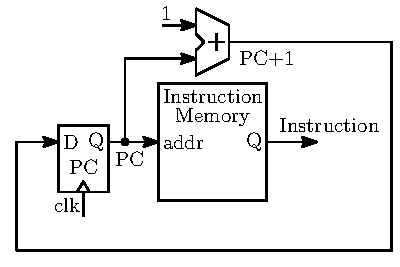
\includegraphics[scale=1.2]{MIPS_design_IF}
  \caption{Basic \ac{PC} datapath.}
  \label{Figure:non_pipelined_IF}
  \end{figure}
  
\end{frame}

\section{R-Type datapath}
% ========================================
% 
% ========================================
\begin{frame}{Custom MIPS design}
\begin{itemize}
\item \Rtype instructions are instructions in which \acs{ALU} operands are retrieved from \ac{RF} and result is stored back in \ac{RF} as well.
\end{itemize}
\vspace{-15pt}
\begin{table}[htbp]
  \label{Table:MIPS_RType_examples}
    \begin{tabular}{l|l|l}
    \hline\hline
    Instruction & Syntax & Meaning \\ \hline
    \code{ADD}  & \code{ADD rd, rs, rt}  & \code{Reg[rd] $\leftarrow$ Reg[rs] + Reg[rt]}\\ \hline
    \code{SUB}  & \code{SUB rd, rs, rt}  & \code{Reg[rd] $\leftarrow$ Reg[rs] - Reg[rt]}\\ \hline
    \code{NAND} & \code{NAND rd, rs, rt} & \code{Reg[rd] $\leftarrow$ $\sim$(Reg[rs] \& Reg[rt])}\\ \hline
    \code{NOR}  & \code{NOR rd, rs, rt}  & \code{Reg[rd] $\leftarrow$ $\sim$(Reg[rs] | Reg[rt])}\\ \hline
    \code{XNOR} & \code{XNOR rd, rs, rt} & \code{Reg[rd] $\leftarrow$ $\sim$(Reg[rs] \^{} Reg[rt])}\\ \hline
    \code{AND}  & \code{AND rd, rs, rt}  & \code{Reg[rd] $\leftarrow$ Reg[rs] \& Reg[rt]}\\ \hline
    \code{OR}   & \code{OR rd, rs, rt}   & \code{Reg[rd] $\leftarrow$ Reg[rs] | Reg[rt]}\\ \hline
    \code{XOR}  & \code{XOR rd, rs, rt}  & \code{Reg[rd] $\leftarrow$ Reg[rs] \^{} Reg[rt]}\\ \hline
    \code{SLL}  & \code{SLL rd, rs, sa}  & \code{Reg[rd] $\leftarrow$ Reg[rs] << sa}\\ \hline
    \code{SRL}  & \code{SRL rd, rs, sa}  & \code{Reg[rd] $\leftarrow$ Reg[rs] >> sa}\\ \hline
    \code{SLA}  & \code{SLA rd, rs, sa}  & \code{Reg[rd] $\leftarrow$ Reg[rs] <<< sa}\\ \hline
    \code{SRA}  & \code{SRA rd, rs, sa}  & \code{Reg[rd] $\leftarrow$ Reg[rs] >>> sa}\\ \hline
    \hline\hline
    \end{tabular}
  \end{table}
\end{frame}

% ========================================
% 
% ========================================
\begin{frame}{R-Type arithmetic/logic instruction}
  \begin{figure}
  \centering
  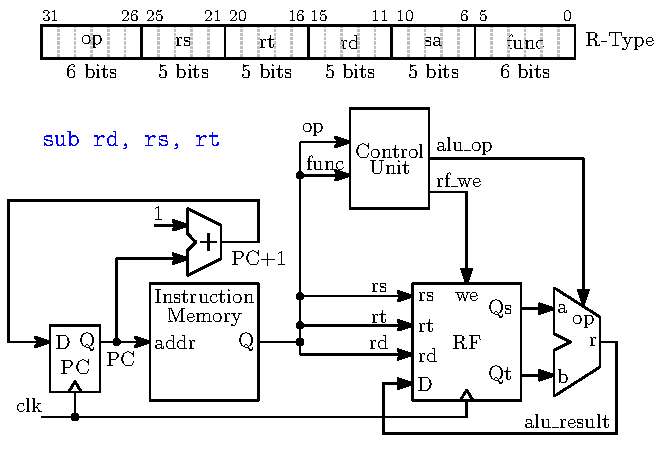
\includegraphics[scale=0.9]{MIPS_design_Rtype_ADD}
  \vspace{-1pt}
  \caption{\ac{uA} of \ac{MIPS} R-Type arithmetic/logic instructions datapath.}
  \label{Figure:non_pipelined_MIPS_Rtype_ADD}
  \end{figure}
\end{frame}

% ========================================
% 
% ========================================
\begin{frame}{R-Type arithmetic/logic instructions datapath}
\begin{itemize}
\item \ac{ALU} takes its operands \codeblue{a} and \codeblue{b} from outputs \codeblue{Qs} and \codeblue{Qt} from \ac{RF}, respectively.
\item Control unit asserts \codeblue{alu\_op} according to value of \codeblue{func} in order to instruct \ac{ALU} the type of operation to be performed, \ie, \codeblue{add}, \codeblue{sub}, \codeblue{and}, \etc. 
\item Control unit asserts \codeblue{rf\_we} in order to write the \codeblue{alu\_result} back into \ac{RF}.
\end{itemize}
\end{frame}

% ========================================
% 
% ========================================
\begin{frame}{R-Type shift instructions datapath}
  \begin{figure}
  \centering
  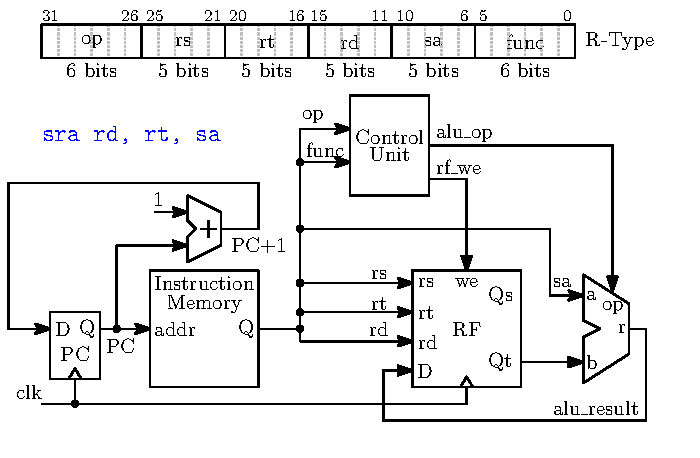
\includegraphics[scale=0.9]{MIPS_design_Rtype_SHIFT}
  \vspace{-3pt}
  \caption{\ac{uA} of \ac{MIPS} R-Type shift instructions datapath.}
  \label{Figure:non_pipelined_MIPS_Rtype_SHIFT}
  \end{figure}
\end{frame}

% ========================================
% 
% ========================================
\begin{frame}{R-Type shift instructions}
\begin{itemize}
\item Input \codeblue{a} in \ac{ALU} represents shift amount \codeblue{sa}.
\item \codeblue{sa} must be zero-extended.
\item \codeblue{rs} and \codeblue{Qs} are not used.
\end{itemize}
\end{frame}

% ========================================
% 
% ========================================
\begin{frame}{R-Type instructions datapath}
\vspace{-6.22pt}
  \begin{figure}
  \centering
  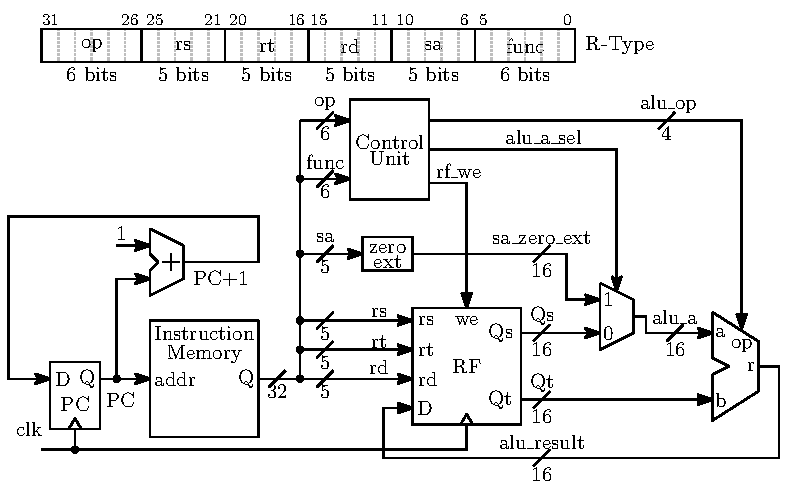
\includegraphics[scale=0.9]{MIPS_design_Rtype_FULL}
  \vspace{-3pt}
  \caption{\ac{uA} of \ac{MIPS} R-Type instructions datapath.}
  \label{Figure:non_pipelined_MIPS_Rtype_FULL}
  \end{figure}
\end{frame}

\section{I-Type datapath}
% ========================================
% 
% ========================================
\begin{frame}{I-Type arithmetic/logic instructions datapath}
\begin{itemize}
\item \Itype instructions use immediate addressing mode.
\end{itemize}
\begin{table}[!htb]
\centering
%\caption{I-Type operations.}
\label{Table:itype_operations}
\begin{tabular}{l|l|l}
\hline\hline
 Instruction & Syntax & Meaning \\
 \hline\hline
    \code{ADDI} & \code{ADDI rt, rs, imm} & \code{Reg[rt] $\leftarrow$ Reg[rs] + imm}    \\\hline
    \code{SUBI} & \code{SUBI rt, rs, imm} & \code{Reg[rt] $\leftarrow$ Reg[rs] - imm}    \\\hline
    \code{ANDI} & \code{ANDI rt, rs, imm} & \code{Reg[rt] $\leftarrow$ Reg[rs] \& imm}   \\\hline
    \code{ORI}  & \code{ORI  rt, rs, imm} & \code{Reg[rt] $\leftarrow$ Reg[rs] | imm}    \\\hline
    \code{XORI} & \code{XORI rt, rs, imm} & \code{Reg[rt] $\leftarrow$ Reg[rs] \^{} imm} \\\hline
    \code{LUI}  & \code{LUI rt, imm}      & \code{Reg[rt] $\leftarrow$ \{imm[7:0], 8'b0\}}   \\\hline
    \code{LLI}  & \code{LLI rt, imm}      & \code{Reg[rt] $\leftarrow$ \{8'b0, imm[7:0]\}}  \\\hline
    \code{LW}   & \code{LW  rt, imm(rs)}  & \code{Reg[rt] $\leftarrow$ Mem[rs+imm]} \\\hline
    \code{SW}   & \code{SWR  rt, imm(rs)} & \code{Mem[rs+imm] $\leftarrow$ Reg[rt]} \\\hline
    \multirow{2}{*}{\code{BEQ}} & \multirow{2}{*}{\code{BEQ rt, rs, imm}}  & \code{if (Reg[rt] == Reg[rs])}  \\
    & & \code{then PC $\leftarrow$ imm} \\\hline
    \multirow{2}{*}{\code{BNE}} & \multirow{2}{*}{\code{BNE rt, rs, imm}}  & \code{if (Reg[rt] != Reg[rs])}  \\
    & & \code{then PC $\leftarrow$ imm} \\\hline
    \hline\hline
 \end{tabular}
\end{table}



\end{frame}

% ========================================
% 
% ========================================
\begin{frame}{I-Type arithmetic/logic instructions datapath}
  \begin{figure}
  \centering
  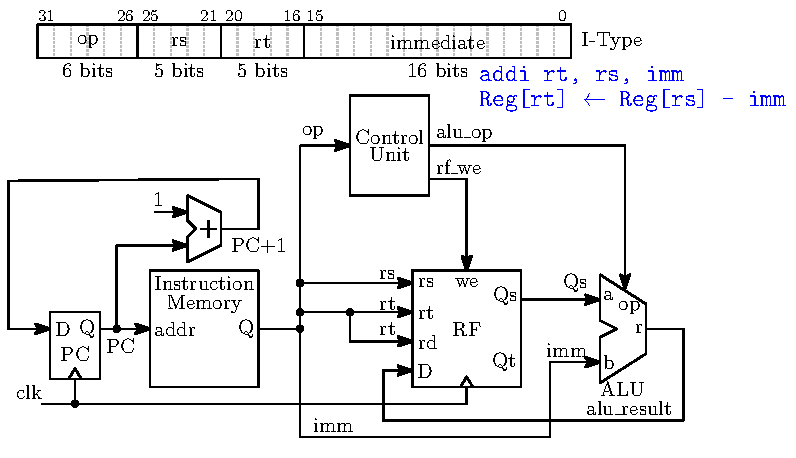
\includegraphics[scale=0.9]{MIPS_design_Itype_ADD}
  \vspace{-3pt}
  \caption{\ac{uA} of a \ac{MIPS} I-Type arithmetic/logic instruction.}
  \label{Figure:non_pipelined_MIPS_Itype_ADD}
  \end{figure}
\end{frame}


% ========================================
% 
% ========================================
%\begin{frame}{I-Type arithmetic/logic instructions datapath}
%\begin{itemize}
%\item Previous slide presented the \Itype datapath for the case when data width is 32 bits.
%\item In our custom \ac{MIPS}, we are using a data width of 16 bits. Hence, the sign extender block %is not necessary.
%\item \codeblue{rd} is not used.
%\item \codeblue{imm} must be sign/zero extended. 
%\end{itemize}
%\end{frame}


% ========================================
% 
% ========================================
\begin{frame}{I-Type load instructions datapath}
  \begin{figure}
  \centering
  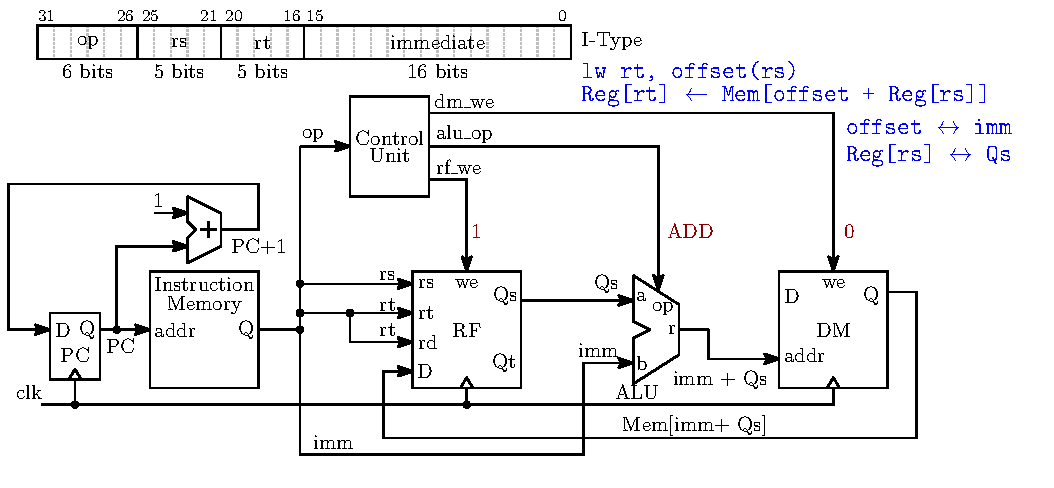
\includegraphics[scale=0.68]{MIPS_design_Itype_LOAD}
  \vspace{-3pt}
  \caption{\ac{uA} of a \ac{MIPS} I-Type load instruction datapath.}
  \label{Figure:non_pipelined_MIPS_Itype_LOAD}
  \end{figure}
\end{frame}

% ========================================
% 
% ========================================
\begin{frame}{I-Type store instructions datapath}
  \begin{figure}
  \centering
  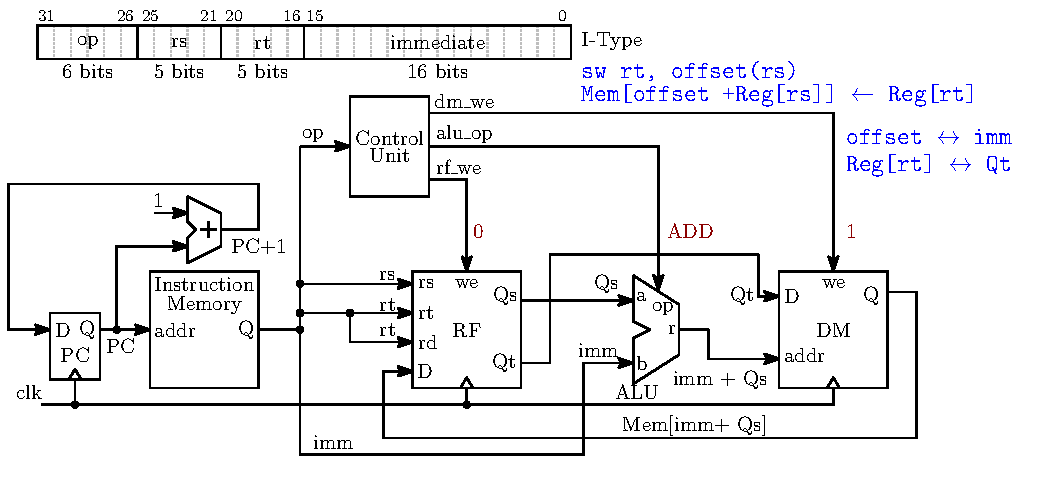
\includegraphics[scale=0.68]{MIPS_design_Itype_STORE}
  \vspace{-3pt}
  \caption{\ac{uA} of a \ac{MIPS} I-Type store instruction datapath.}
  \label{Figure:non_pipelined_MIPS_Itype_STORE}
  \end{figure}
\end{frame}

% ========================================
% 
% ========================================
\begin{frame}{I-Type load/store instructions}
\begin{itemize}
\item \ac{ALU} will perform calculations in order to find the displacement address to read/write data from/to.
\begin{itemize}
\item \codeblue{lw rt, offset(rs)} is equivalent to
\begin{itemize}
\item[] \codeblue{Reg[rt] $\leftarrow$ Mem[offset+Reg[rs]]}
\end{itemize} 
\item[] \codeblue{sw rt, offset(rs)} is equivalent to 
\begin{itemize}
\item[] \codeblue{Mem[offset+Reg[rs]] $\leftarrow$ Reg[rt]}
\end{itemize}
\end{itemize}
\item Control unit provides a \codeblue{dm\_we} signal, which is a write enable for reading/writing from \ac{DM}.
\end{itemize}
\end{frame}

% ========================================
% 
% ========================================
\begin{frame}{I-Type conditional branch instructions}
  \begin{figure}
  \centering
  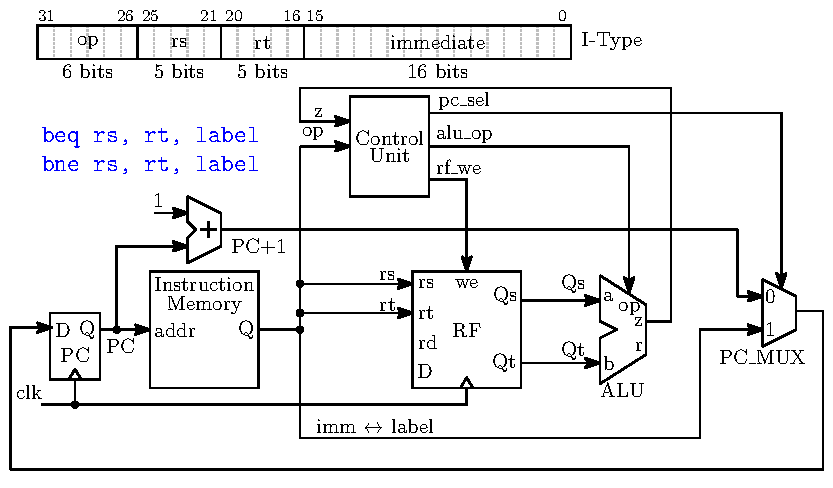
\includegraphics[scale=0.78]{MIPS_design_Itype_BRANCH}
  \vspace{-3pt}
  \caption{\ac{uA} of a \ac{MIPS} I-Type conditional branch instruction.}
  \label{Figure:non_pipelined_MIPS_Itype_BRANCH}
  \end{figure}
\end{frame}

% ========================================
%
% ========================================
\begin{frame}{I-Type load/store instructions}
\begin{itemize}
\item Contents of \codeblue{rs} and \codeblue{rt} are compared in order to determine whether to branch or not.
\item If the branch is taken, \ac{PC} is updated with an \code{imm} value, which is the target address.
\item There is no write-back to \ac{RF}.
\end{itemize}
\end{frame}

\section{J-Type datapath}
% ========================================
% 
% ========================================
\begin{frame}{J-Type instructions}
  \begin{figure}
  \centering
  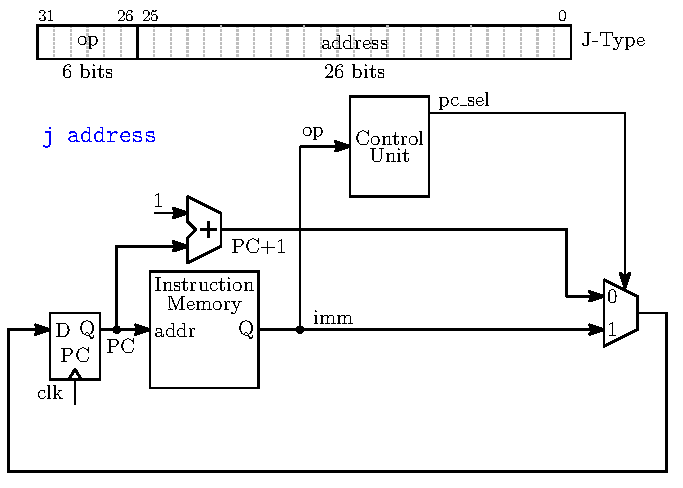
\includegraphics[scale=0.78]{MIPS_design_Jtype_JUMP}
  \vspace{-3pt}
  \caption{\ac{uA} of a \ac{MIPS} J-Type jump instruction.}
  \label{Figure:non_pipelined_MIPS_Jtype_JUMP}
  \end{figure}
\end{frame}

\end{document}
